\documentclass[12pt,a4paper]{article}
\usepackage[utf8]{inputenc}
\usepackage[margin=1in]{geometry}
\usepackage{amsmath,amssymb}
\usepackage{booktabs}
\usepackage{float}
\usepackage{parskip}
\usepackage{graphicx}
\usepackage{caption}
\usepackage{fancyhdr}

\begin{document}

\pagestyle{fancy}
\fancyhf{}
\fancyhead[L]{
\includegraphics[height=1cm]{IIITB-COMET-Logo.png}}
\fancyhead[R]{Name: P.Muskan\\ID: cometfwc035}

\begin{center}
    {\Large \textbf{GATE 2010 (EC) – Question 42 }}\\[4pt]
    \rule{0.9\linewidth}{0.4pt}
\end{center}

\section*{Question}
\begin{figure}[H]
	\centering
	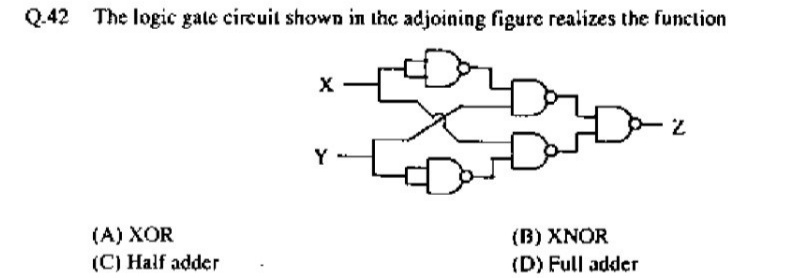
\includegraphics[width=0.8\linewidth]{question42.png}
\end{figure}
The logic gate circuit shown in the question (two-input network with inputs $X$ and $Y$ feeding a small network of NAND/NOT gates, output $Z$) realizes which function?
\begin{enumerate}
    \item[(A)] XOR \qquad
    \item[(B)] XNOR \qquad
    \item[(C)] Half adder \qquad
    \item[(D)] Full adder
\end{enumerate}

\section*{Short Answer}
\[
\boxed{\text{XOR (Option (A))}}
\]

\section*{Solution (Logic Derivation)}
Carefully inspecting the network and its gate interconnections (or deriving the expression from the small sub-networks) shows the output is high when exactly one of the inputs is high.

A canonical algebraic expression for the XOR function is:
\[
Z = X \wedge Y = \overline{X}Y + X\overline{Y}.
\]

You can also derive this from the gate-level structure by identifying two paths that implement $\overline{X}Y$ and $X\overline{Y}$ and then OR-ing them.

\section*{Truth Table}
\begin{table}[H]
\centering
\begin{tabular}{@{}c c c@{}}
\toprule
$X$ & $Y$ & $Z = X \wedge Y$ \\
\midrule
0 & 0 & 0 \\
0 & 1 & 1 \\
1 & 0 & 1 \\
1 & 1 & 0 \\
\bottomrule
\end{tabular}
\caption{Truth table for XOR operation}
\end{table}

\section*{Boolean Algebra / Alternate forms}
\[
X \wedge Y = \overline{X}Y + X\overline{Y}.
\]
Using product-of-sums:
\[
X \wedge Y = (X + Y)\cdot(\overline{X} + \overline{Y}) \quad\text{(one can transform forms with De Morgan).}
\]

\section*{Hardware Implementation with 7474 and 7447 ICs}
A complete implementation of the XOR function with storage and display capabilities uses:

\begin{itemize}
  \item 2× \textbf{7474} — Dual D-type Flip Flop (to store the XOR result)
  \item 1× \textbf{7447} — BCD to 7-segment decoder (to drive the display)
  \item 1× \textbf{Common Anode 7-segment Display} (to show the output)
  \item 7× \textbf{220 ohms resistors} (for current limiting on the display)
  \item Arduino Uno (to provide clock signal)
  \item Breadboard, jumper wires
  \item 5V regulated supply
\end{itemize}

\subsection*{IC Pin Connections}

\subsubsection*{7474 (D-Flip Flop) - 14-pin DIP}
\begin{itemize}
  \item VCC: Pin 14 to +5V
  \item GND: Pin 7 to Ground
  \item Clock: Pin 3 (from Arduino D13)
  \item D Input: Pin 2 (from 7486 Pin 3)
  \item Q Output: Pin 5 (to 7447 Pin 7)
  \item Preset (PR): Pin 4 to +5V
  \item Clear (CLR): Pin 1 to +5V
\end{itemize}

\subsubsection*{7447 (BCD-to-7-Segment Decoder) - 16-pin DIP}
\begin{itemize}
  \item VCC: Pin 16 to +5V
  \item GND: Pin 8 to Ground
  \item Input D: Pin 7 (from 7474 Pin 5)
  \item Inputs C, B, A: Pins 1, 2, 6 to GND (for 0 input)
  \item Outputs: Pins 9-15 to Seven Segment Display through 220 ohms resistors
\end{itemize}

\subsubsection*{Seven Segment Display (Common Anode)}
\begin{itemize}
  \item a: Through resistor to 7447 Pin 13
  \item b: Through resistor to 7447 Pin 12
  \item c: Through resistor to 7447 Pin 11
  \item d: Through resistor to 7447 Pin 10
  \item e: Through resistor to 7447 Pin 9
  \item f: Through resistor to 7447 Pin 15
  \item g: Through resistor to 7447 Pin 14
  \item Common Anode: To +5V
\end{itemize}

\section*{Arduino Code for Clock Generation}
\begin{verbatim}
// XOR Implementation with 7474 and 7447 ICs
// Inputs: X (pin 2), Y (pin 3)
// Clock output: pin 13 to 7474

const int inputX = 2;
const int inputY = 3;
const int clockPin = 13;

void setup() {
  pinMode(inputX, INPUT);
  pinMode(inputY, INPUT);
  pinMode(clockPin, OUTPUT);
  
  // Initialize serial communication for monitoring
  Serial.begin(9600);
}

void loop() {
  // Read inputs
  int X = digitalRead(inputX);
  int Y = digitalRead(inputY);
  
  // Generate clock signal
  digitalWrite(clockPin, HIGH);
  delay(500);
  digitalWrite(clockPin, LOW);
  delay(500);
  
  // Display status
  Serial.print("X: ");
  Serial.print(X);
  Serial.print(" | Y: ");
  Serial.print(Y);
  Serial.print(" | XOR Output: ");
  Serial.println(X != Y ? "1" : "0");
}
\end{verbatim}

\section*{Operation Explanation}
\begin{enumerate}
  \item The result is stored in the 7474 D-flip flop on the rising edge of the clock
  \item The stored value is displayed on the seven-segment display via the 7447 decoder
  \item Since we're only displaying 0 or 1, we only use the D input of the 7447 (pin 7)
  \item The Arduino provides the clock signal and can be used to monitor the operation
\end{enumerate}

\section*{Test Procedure}
\begin{enumerate}
  \item Connect all components as described
  \item Upload the Arduino code
  \item Apply different combinations of X and Y inputs (0/1)
  \item Observe the seven-segment display showing 1 when inputs differ, 0 when they match
  \item The serial monitor will display the current input values and XOR result
\end{enumerate}

\begin{figure}[H]
\centering
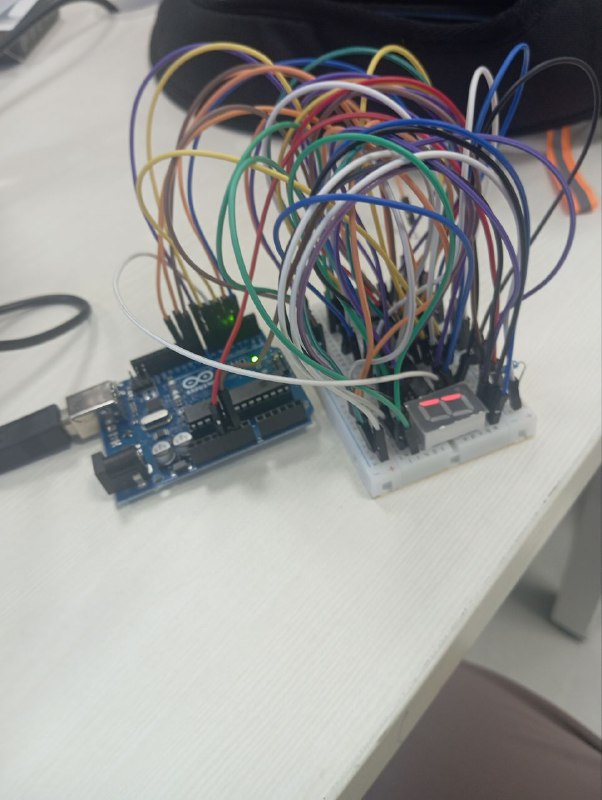
\includegraphics[width=0.8\linewidth]{output.png}
\end{figure}

\section*{Conclusion}
The network implements the exclusive-OR function:
\[
\boxed{Z = X \wedge Y = \overline{X}Y + X\overline{Y}}
\]
This outputs logic 1 exactly when the inputs differ. The implementation with 7486, 7474, and 7447 ICs demonstrates how to combine combinational logic, sequential elements, and display drivers to create a complete digital system.

\end{document}
